\documentclass[handout]{beamer}

\usepackage[frenchb]{babel}
\usepackage[T1]{fontenc}
\usepackage[utf8x]{inputenc}
 
\usetheme{Berkeley}
\usecolortheme{crane}
\useinnertheme{rounded}

\newcommand{\derPar}[2]{\frac{\partial #1}{\partial #2}}

\title[PFE]{Projet de Fin d'Étude : \\ Propagation d'un pathogène dans un champ de blé}
\author{Alexandre \bsc{Vieira}}
\institute{INSA de Rouen}
\date{\today}


\AtBeginSection[]
{
	\begin{frame}
		\frametitle{Sommaire}
		\tableofcontents[currentsection, hideothersubsections]
	\end{frame}
}

\begin{document}

\begin{frame}
\titlepage
\end{frame}

\begin{frame}
	\frametitle{Sommaire}
	\tableofcontents
\end{frame}

\section[Modèle]{Modèle mathématique étudié}
\subsection[Diff. modèles]{Différents modèles}
\begin{frame}
	\frametitle{Modèles de propagation}
Modèle SI :
\[\begin{array}{c c c}
	\frac{dS}{dt}&=&-\beta SI\\
	\frac{dI}{dt}&=&\beta SI
\end{array}\]
Modèle de contact distribué :
\begin{equation} \label{eqKot}
	\derPar{I}{t}(x,t)=\beta(x)(N-I(x,t))\int_{\mathbb{R}}k(x,y)I(y,t) dy
\end{equation}
Modèle avec mouvement de population
\begin{equation}
	\derPar{I}{t}(x,t)=\beta(x)(N-I(x,t))-DI(x,t)+D\int_{\mathbb{R}}k(x,y)I(y,t) dy
\end{equation}
\end{frame}

\subsection[Vitesse]{Étude de la vitesse de propagation}
\begin{frame}
	\frametitle{Vitesse de propagation}
Vitesse bornée par le modèle linéaire :
\[\derPar{I}{t}=\beta(x)N\int_{\mathbb{R}}k(x,y)I(y,t) dt\]
Condition initiale bornée par une exponentielle :
\[I_0(x,0)\leq Ae^{-\theta x}\]	
Vitesse bornée par
\begin{equation}\label{bornVit}
	c=\beta(x)\inf_{\theta>0}\frac{M(\theta)}{\theta}
\end{equation}
Conjecture : sous certaines hypothèses, vitesse du modèle complet = vitesse du modèle linéaire.
\end{frame}

\subsection[Forme]{Étude de la forme du front d'onde}
\begin{frame}
	\frametitle{Forme du front d'onde}
	Raisonnement par perturbations. Forme du front d'onde à l'ordre 0 donné par :
	\[I(z)=\frac{1}{1+\exp\left(\beta\frac{z}{c}\right)}\]
\begin{figure}[!h]
	\centering
	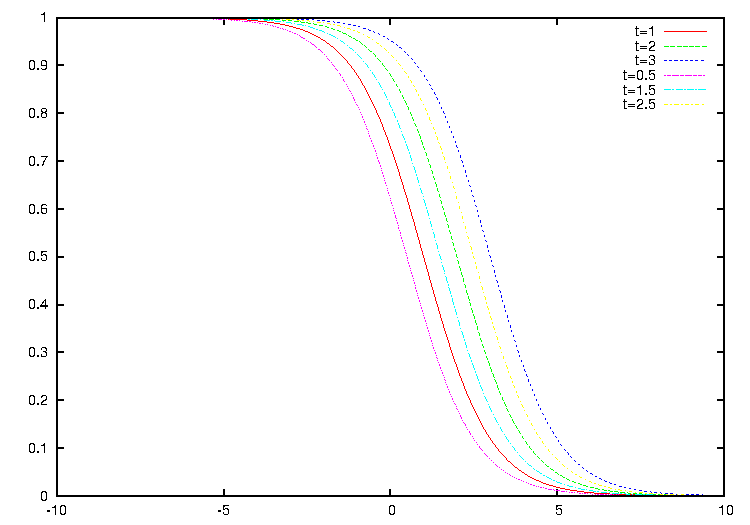
\includegraphics[scale=0.5]{img/plotShape.pdf}
\caption{Forme approchée du front à l'ordre 0 : $\beta=1$, $c=1$}
\label{plotShape}
\end{figure}
\end{frame}


\section[Simulation]{Simulation numérique}
\subsection[Simplification]{Simplification de l'équation}
\begin{frame}
	\frametitle{Forme du front d'onde}
\[\frac{\partial I}{\partial t}(x,t) =\beta(x)N\sum_{n=0}^{+\infty} \frac{(-1)^n\mu_n}{n!} \frac{\partial^n I}{\partial x^n}(x,t)\]
\begin{equation}\label{approx}
	\derPar{I}{t}(x,t)=\beta(x)\left(I(x,t)+\frac{\mu_2}{2}\derPar{{}^2I}{x^2}\right)
\end{equation}

\end{frame}

\subsection[Résultats]{Résultats numériques}
\begin{frame}
	\frametitle{Cadre, résultats et analyse}
	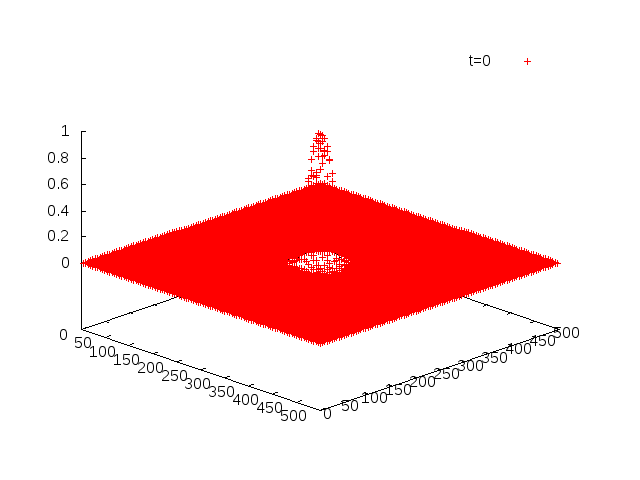
\includegraphics[scale=0.2]{img/anim1-10-1.png}
	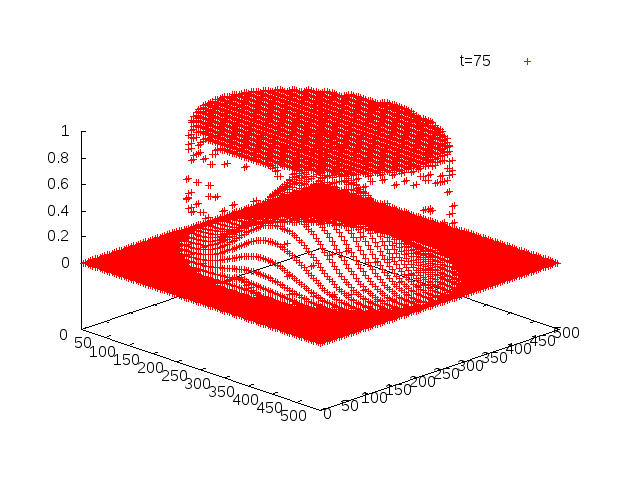
\includegraphics[scale=0.2]{img/anim1-10-150.png}\\
	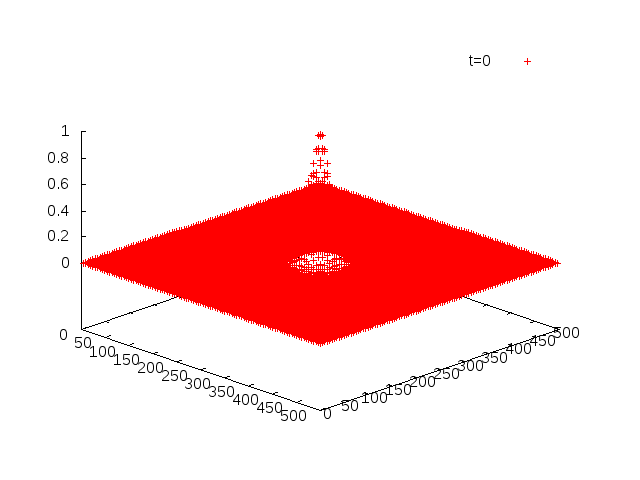
\includegraphics[scale=0.2]{img/anim1-80-1.png}
	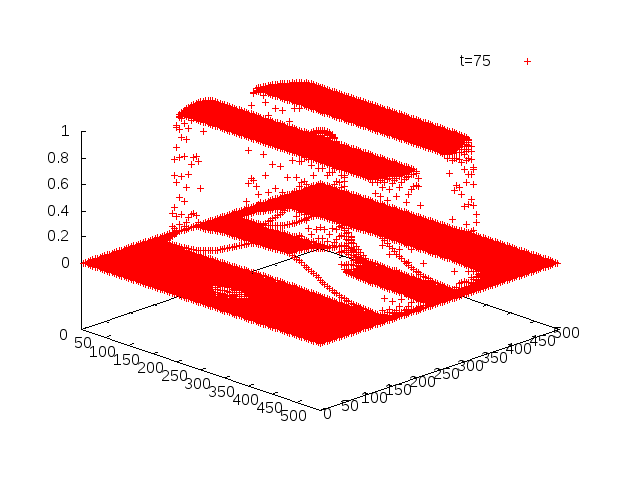
\includegraphics[scale=0.2]{img/anim1-80-150.png}
\end{frame}

\begin{frame}
	\frametitle{Cadre, résultats et analyse}
	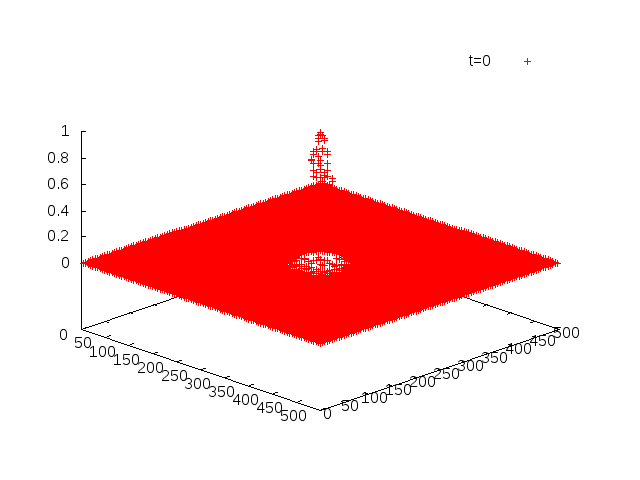
\includegraphics[scale=0.2]{img/anim2-10-1.png}
	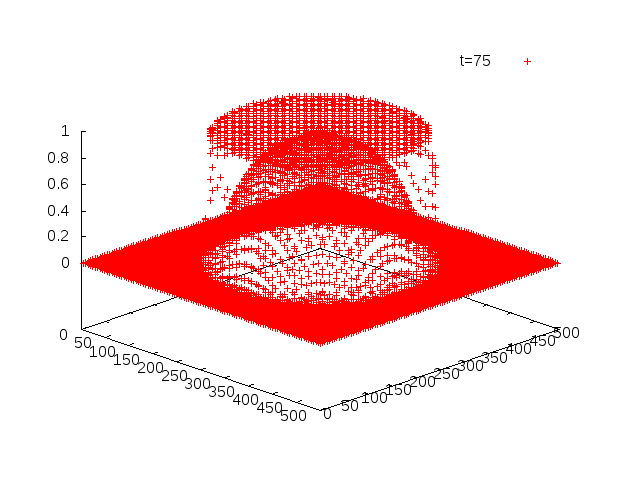
\includegraphics[scale=0.2]{img/anim2-10-150.png}\\
	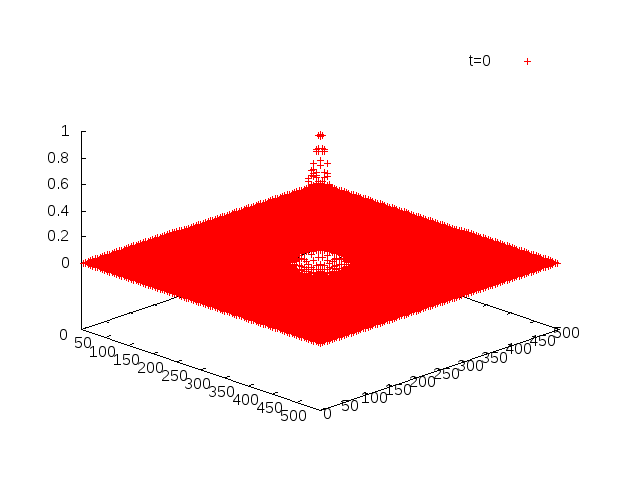
\includegraphics[scale=0.2]{img/anim2-80-1.png}
	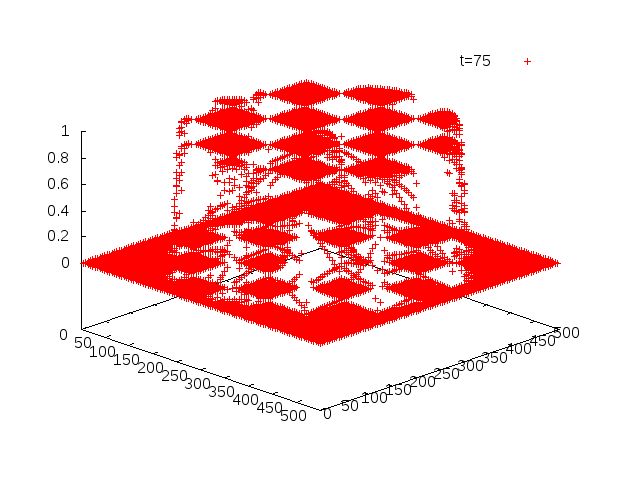
\includegraphics[scale=0.2]{img/anim2-80-150.png}
\end{frame}

\section[Limite propagation]{Problème de décision : limiter la propagation du pathogène}
\subsection[Problème]{Formulation du problème}
\begin{frame}
	\frametitle{Problème de décision}
\[\begin{array}{c c}
	\text{Maximiser } &t\\
	\text{tel que } & \left\{\begin{array}{c}
			\frac{1}{mes(\Omega)}\int_\Omega I(x,t) dx > 0,5\\
			r_1\leq R\leq r_2\\
			x_{\mu}>\alpha
			\end{array}\right.
\end{array}\]
Difficile à traiter.
\end{frame}

\subsection[Théorique]{Considérations théoriques}
\begin{frame}
	\frametitle{Largeur du front d'onde}
\begin{equation}
	c=\beta\underbrace{\inf_{\theta>0} \frac{M(\theta)}{\theta} }_{=K}= \beta K
\end{equation}
Approximation à l'ordre 0 de la forme du front d'onde :
\begin{equation}
	I(z)=\frac{1}{1+\exp\left(\frac{\beta}{c}z\right)}
\end{equation}
$\Rightarrow$ Largeur du front d'onde :
\begin{equation}
	w=\frac{c}{\beta}=\frac{\beta K}{\beta}=K \text{ constante indépendante de }\beta
\end{equation}
\begin{center}$x_{\mu}<w$ ou $x_{\mu}>w$ ? \end{center}
\end{frame}

\subsection[Numérique]{Simulation numérique}
\begin{frame}
	\frametitle{Résulats}
\begin{figure}[!h]
\centering
	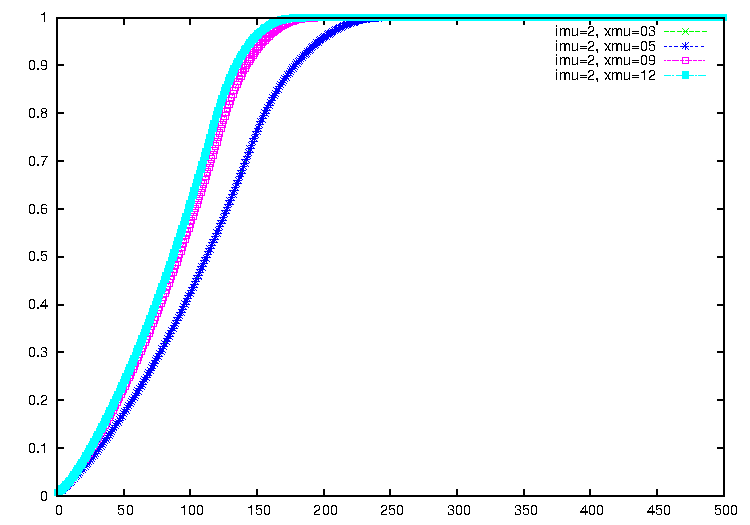
\includegraphics[scale=0.75]{img/plot2-2.pdf}
\end{figure}
\end{frame}

\end{document}
